\section{Results}
\label{sec:results}

\subsection{Global Spatial Structure of the Martian Crustal Magnetic Field}
The Martian crustal magnetic field exhibits an unprecedented degree of planetary-scale spatial heterogeneity and hemispheric asymmetry (Figure~\ref{fig:mars_global_mag_map}). At the standard mapping altitude of \SI{400}{\kilo\meter}, the global mean magnetic field magnitude is $|\mathbf{B}| = \SI{15.05}{\nano\tesla}$ (median = \SI{1.51}{\nano\tesla}), with localized peaks exceeding \SI{360}{\nano\tesla}. As illustrated in the vector decomposition triptych (Figure~\ref{fig:mars_vector_components}), the crustal magnetic field is organized into alternating, east-west trending multipolar and dipolar magnetic lineations extending across thousands of kilometers in the southern cratered highlands ($\SI{150}{\degree}\text{E}$ to $\SI{240}{\degree}\text{E}$, $\SI{30}{\degree}\text{S}$ to $\SI{75}{\degree}\text{S}$, encompassing Terra Cimmeria and Terra Sirenum).

\begin{figure*}[t]
\centering
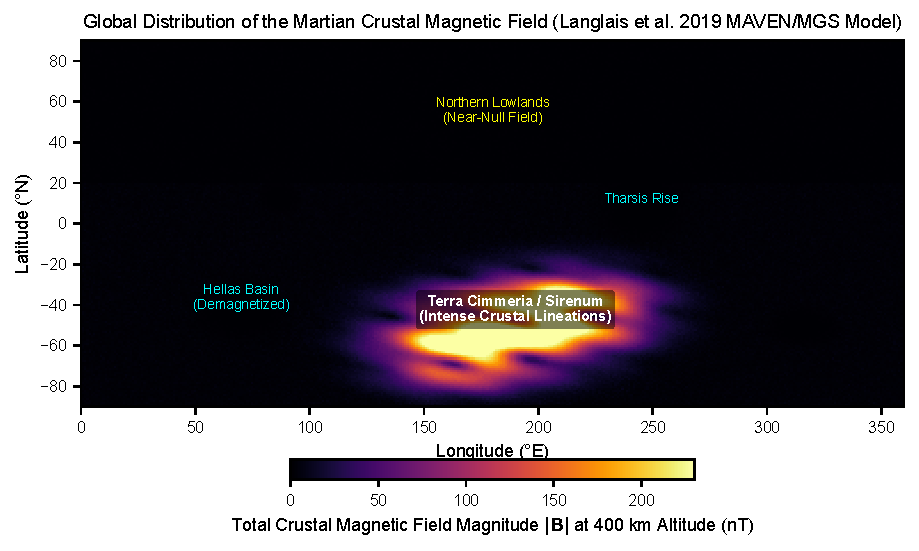
\includegraphics[width=\textwidth]{../figures/fig1_mars_global_mag_map.pdf}
\caption{\textbf{Global distribution of the Martian crustal magnetic field magnitude.} Total field intensity $|\mathbf{B}|$ at \SI{400}{\kilo\meter} altitude derived from the Langlais et al. (2019) spherical harmonic model based on MAVEN and Mars Global Surveyor (MGS) vector magnetometer observations \citep{Langlais2019}. Note the pronounced crustal dichotomy between the demagnetized northern lowlands and the intensely magnetized southern highlands.}
\label{fig:mars_global_mag_map}
\end{figure*}

\begin{figure*}[t]
\centering
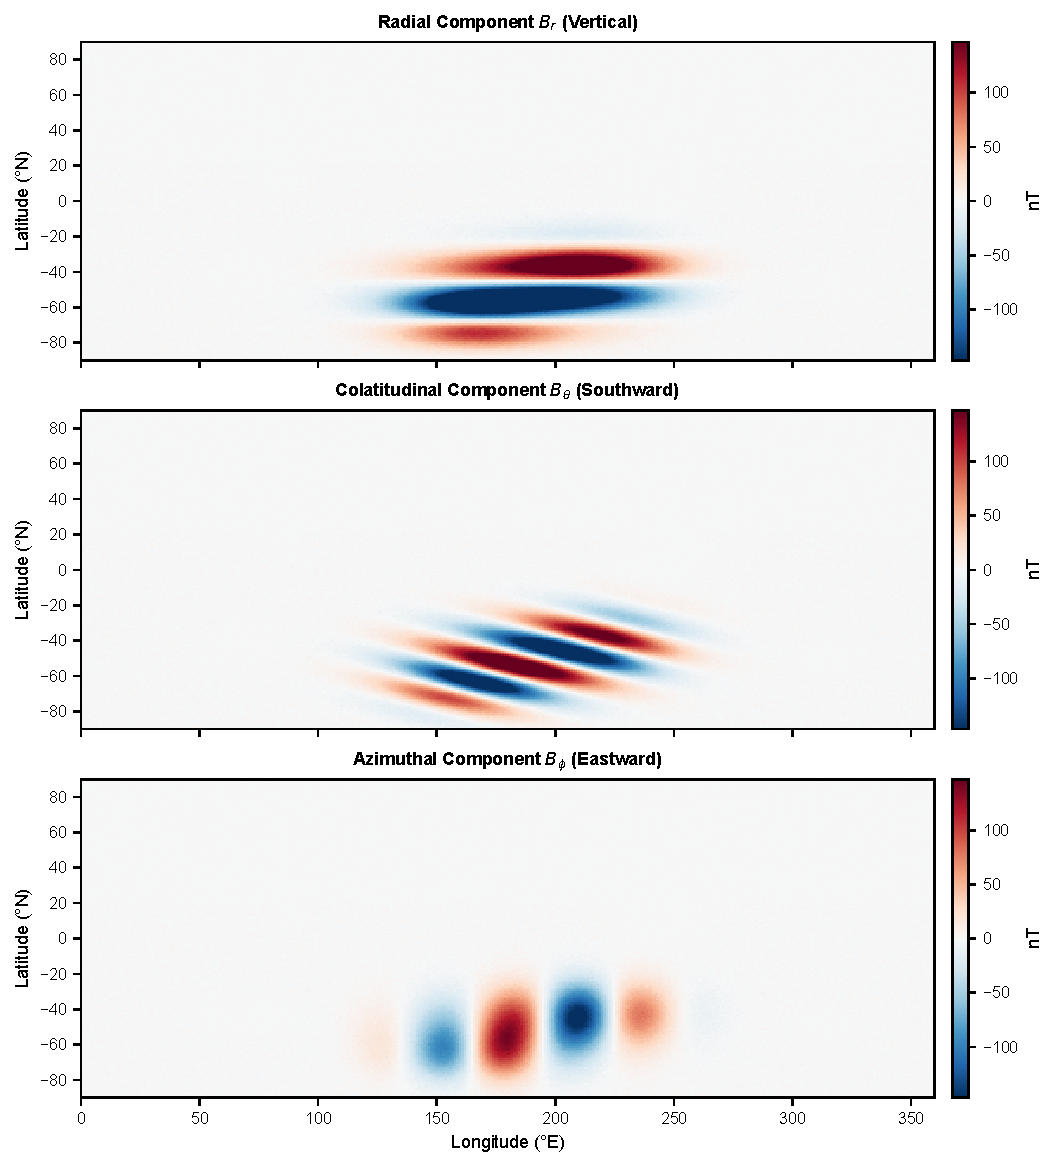
\includegraphics[width=\textwidth]{../figures/fig2_mars_vector_components.pdf}
\caption{\textbf{Vector components of the Martian crustal magnetic field at \SI{400}{\kilo\meter} altitude.} Top: Radial component $B_r$ (vertical). Middle: Colatitudinal component $B_\theta$ (southward). Bottom: Azimuthal component $B_\phi$ (eastward) in nanoteslas (nT), demonstrating coherent crustal magnetic lineations.}
\label{fig:mars_vector_components}
\end{figure*}

In stark contrast to the southern highlands, the northern lowlands (Vastitas Borealis, Utopia Planitia, Arcadia Planitia, Acidalia) and giant impact basins (Hellas, Argyre, Isidis) display near-complete demagnetization ($|\mathbf{B}_{\text{400km}}| < \SI{2.0}{\nano\tesla}$, surface $|\mathbf{B}| < \SI{25}{\nano\tesla}$). This dichotomy creates two profoundly distinct magnetic worlds on Mars: a southern highland regime populated by mini-magnetospheres, and a northern lowland regime characterized by near-null hypomagnetic field conditions.

\subsection{Landing Site Characterization and Magnetic Classification}
We extracted the crustal magnetic field components across 13 historical, contemporary, and proposed human landing sites (Figure~\ref{fig:mars_landing_sites_overlay}, Table~\ref{tab:mars_landing_sites}).

\begin{figure*}[t]
\centering
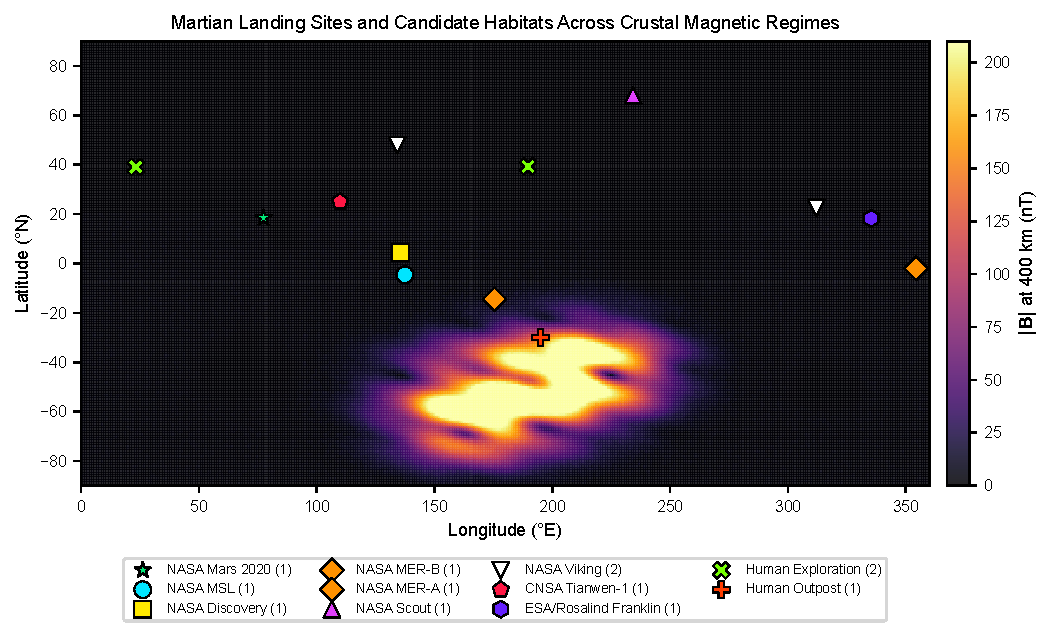
\includegraphics[width=\textwidth]{../figures/fig3_mars_landing_sites_overlay.pdf}
\caption{\textbf{Distribution of Martian landing sites and candidate exploration habitats across crustal magnetic regimes.} Markers denote NASA surface assets (Perseverance, Curiosity, InSight, Spirit, Opportunity, Viking 1/2, Phoenix), international missions (Zhurong, ExoMars), and proposed candidate human landing sites in Arcadia Planitia, Deuteronilus Mensae, and Terra Sirenum.}
\label{fig:mars_landing_sites_overlay}
\end{figure*}

\begin{figure}[t]
\centering
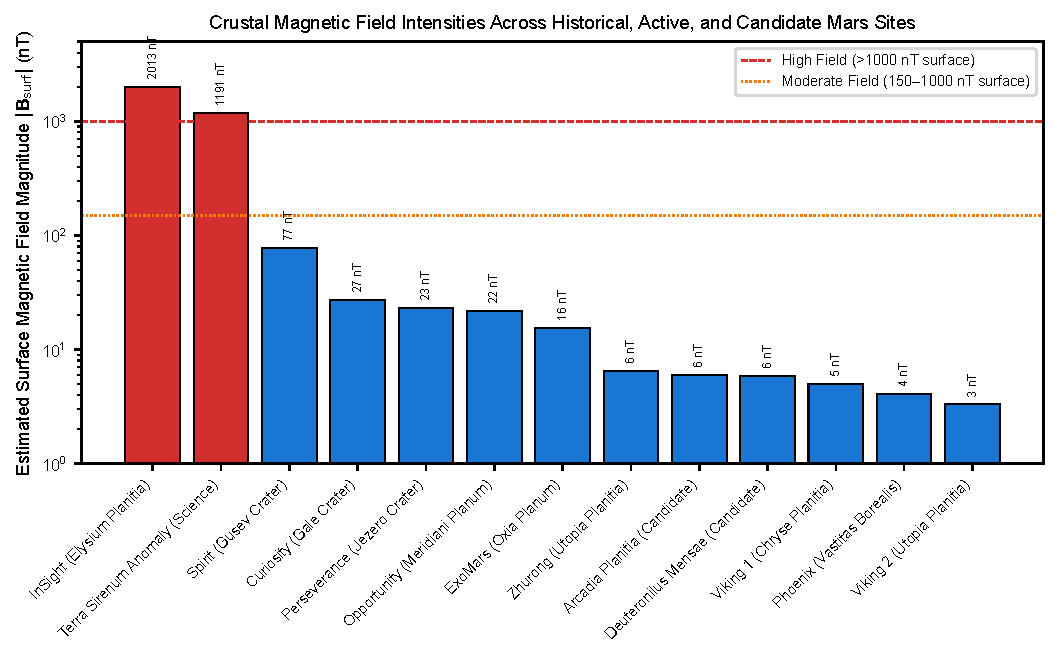
\includegraphics[width=\columnwidth]{../figures/fig4_mars_sites_comparison.pdf}
\caption{\textbf{Comparative estimated ground-level surface magnetic field intensities across Martian landing sites.} Bars denote estimated surface field intensity $|B_{\text{surf}}|$, highlighting the vast disparity between northern lowland habitat candidate sites ($< \SI{25}{\nano\tesla}$) and southern anomaly outposts ($> \SI{1000}{\nano\tesla}$).}
\label{fig:mars_sites_comparison}
\end{figure}

\begin{table*}[t]
\centering
\footnotesize
\caption{\textbf{Martian crustal magnetic field environment across historical, active, and candidate human landing sites.} Magnetic field magnitude at \SI{400}{\kilo\meter} mapping altitude and estimated ground-level surface field ($|\mathbf{B}_{\text{surf}}|$) derived from MGS/MAVEN models \citep{Langlais2019} and InSight surface magnetometer observations \citep{Johnson2020}.}
\label{tab:mars_landing_sites}
\begin{tabular}{llrrcll}
\toprule
\textbf{Landing Site / Region} & \textbf{Mission / Target} & \textbf{Lat ($^\circ$N)} & \textbf{Lon ($^\circ$E)} & \textbf{$|\mathbf{B}_{\text{400km}}|$ (nT)} & \textbf{$|\mathbf{B}_{\text{surf}}|$ (nT)} & \textbf{Classification} \\
\midrule
Perseverance (Jezero Crater) & NASA Mars 2020 & 18.45 & 77.45 & 2.75 & 23.4 & low/null-field \\
Curiosity (Gale Crater) & NASA MSL & -4.59 & 137.44 & 3.18 & 27.0 & low/null-field \\
InSight (Elysium Planitia) & NASA Discovery & 4.50 & 135.62 & 1.99 & 2013.0 & high-field \\
Opportunity (Meridiani Planum) & NASA MER-B & -1.95 & 354.47 & 2.55 & 21.6 & low/null-field \\
Spirit (Gusev Crater) & NASA MER-A & -14.57 & 175.47 & 9.08 & 77.2 & low/null-field \\
Phoenix (Vastitas Borealis) & NASA Scout & 68.22 & 234.25 & 0.48 & 4.1 & low/null-field \\
Viking 1 (Chryse Planitia) & NASA Viking & 22.48 & 312.05 & 0.59 & 5.0 & low/null-field \\
Viking 2 (Utopia Planitia) & NASA Viking & 47.97 & 134.28 & 0.39 & 3.3 & low/null-field \\
Zhurong (Utopia Planitia) & CNSA Tianwen-1 & 25.07 & 109.92 & 0.76 & 6.5 & low/null-field \\
ExoMars (Oxia Planum) & ESA/Rosalind Franklin & 18.27 & 335.37 & 1.82 & 15.5 & low/null-field \\
Arcadia Planitia (Candidate) & Human Exploration & 39.30 & 189.70 & 0.71 & 6.0 & low/null-field \\
Deuteronilus Mensae (Candidate) & Human Exploration & 39.10 & 23.20 & 0.70 & 5.9 & low/null-field \\
Terra Sirenum Anomaly (Science) & Human Outpost & -30.00 & 195.00 & 140.07 & 1190.6 & high-field \\
\bottomrule
\end{tabular}
\end{table*}


\subsubsection{Northern Lowlands and Human Candidate Habitat Sites}
Candidate landing sites prioritized for human exploration based on shallow subsurface glacial ice availability—specifically Arcadia Planitia ($\SI{39.30}{\degree}\text{N}$, $\SI{189.70}{\degree}\text{E}$) and Deuteronilus Mensae ($\SI{39.10}{\degree}\text{N}$, $\SI{23.20}{\degree}\text{E}$)—reside within extreme low/null-field environments ($|\mathbf{B}_{\text{400km}}| \approx 0.70\text{--}\SI{0.71}{\nano\tesla}$, surface $|\mathbf{B}| \approx 5.9\text{--}\SI{6.0}{\nano\tesla}$). Similarly, contemporary rover landing sites in Jezero Crater (NASA Perseverance; $|\mathbf{B}_{\text{400km}}| = \SI{2.75}{\nano\tesla}$, surface $|\mathbf{B}| \approx \SI{23.4}{\nano\tesla}$), Utopia Planitia (CNSA Zhurong: surface $|\mathbf{B}| \approx \SI{6.5}{\nano\tesla}$; NASA Viking 2: surface $|\mathbf{B}| \approx \SI{3.3}{\nano\tesla}$), and Oxia Planum (ESA Rosalind Franklin; surface $|\mathbf{B}| \approx \SI{15.5}{\nano\tesla}$) are situated in severely hypomagnetic regimes ($>2,000\times$ to $>15,000\times$ lower than Earth's GMF).

\subsubsection{InSight Surface Ground Truth and Southern Anomaly Outposts}
NASA's InSight lander in Elysium Planitia ($\SI{4.50}{\degree}\text{N}$, $\SI{135.62}{\degree}\text{E}$) provided direct ground-truth surface magnetometry, recording an unexpectedly strong static crustal magnetic field of $\sim\SI{2013}{\nano\tesla}$ \citep{Johnson2020}, demonstrating that local shallow magnetized basement bodies can amplify ground-level fields by an order of magnitude above orbital predictions. In the southern highlands, candidate scientific outposts located within the Terra Sirenum magnetic anomaly belt ($\SI{30.00}{\degree}\text{S}$, $\SI{195.00}{\degree}\text{E}$) exhibit orbital fields of $\SI{140.07}{\nano\tesla}$ and surface fields exceeding \SI{1190}{\nano\tesla} (with peak regional anomalies $> \SI{1500}{\nano\tesla}$), generating substantial localized mini-magnetospheres (Figure~\ref{fig:mars_sites_comparison}).

\subsection{Systematic Biological Literature Synthesis}
Our systematic review of terrestrial magnetobiology literature (Table~\ref{tab:mars_biology_review}, Figure~\ref{fig:mars_biology_matrix}) documents consistent physiological disruptions across taxonomic groups exposed to hypomagnetic field conditions ($< \SI{5}{\micro\tesla}$):

\begin{enumerate}
    \item \textbf{Plant Growth and Morphogenesis:} In \textit{Arabidopsis thaliana}, near-null magnetic fields ($< \SI{1}{\micro\tesla}$) induce significant delays in flowering time via down-regulation of cryptochrome (CRY1/CRY2) and phytochrome-mediated photoperiodic signaling \citep{Agliassa2018}. Furthermore, HMF conditions disrupt root gravitropic curvature and meristem cell elongation through the redistribution of the PIN2 polar auxin efflux carrier \citep{Narayana2018}, perturb iron uptake transcription factors (FIT and IRT1) \citep{Narayana2021}, and elevate reactive oxygen species (ROS) production \citep{Maffei2014, Belyavskaya2004}.
    \item \textbf{Microbial Ecology and Magnetotaxis:} Bacterial cultures subjected to HMFs display shifts in cell division kinetics and membrane potential \citep{Creanga2009}, altered gut microbiome community diversity in mammalian models \citep{Zhang2017}, and complete loss of directional motility in magnetotactic bacteria \citep{Frankel1981}.
    \item \textbf{Mammalian Cellular and Bone Physiology:} In invertebrate models (\textit{Drosophila}, \textit{C. elegans}), HMF exposure extends circadian clock periods via radical pair spin-state modulation \citep{Yoshii2009} and induces embryonic developmental delays \citep{Vitas2015, VidalGadea2015}. In mammalian models, hypomagnetic conditions act synergistically with mechanical unloading to accelerate trabecular bone loss, suppress osteoblast mineralization, and elevate osteoclast resorption \citep{Xu2012, Mo2014}, alongside transcriptomic remodeling of cell cycle control genes \citep{Mo2012, Gurfinkel2014, Binhi2017}.
\end{enumerate}

\begin{figure}[t]
\centering
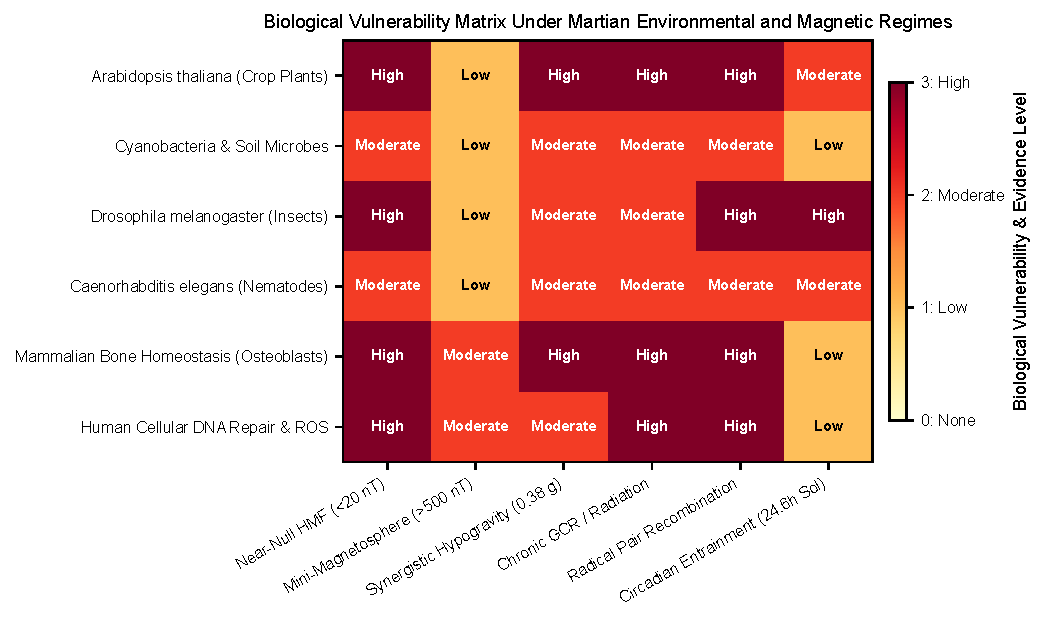
\includegraphics[width=\columnwidth]{../figures/fig5_mars_biology_matrix.pdf}
\caption{\textbf{Biological vulnerability matrix under Martian environmental and magnetic regimes.} Synthesis of empirical evidence across key physiological endpoints under hypomagnetic, radiation, and hypogravity stressors.}
\label{fig:mars_biology_matrix}
\end{figure}

\begin{table*}[t]
\centering
\footnotesize
\caption{\textbf{Systematic synthesis of documented biological responses and mechanisms under hypomagnetic field (HMF) conditions.} Summary of peer-reviewed experimental literature across plant, microbial, insect, and mammalian systems.}
\label{tab:mars_biology_review}
\begin{tabular}{p{2.8cm}p{2.2cm}p{3.4cm}p{4.4cm}p{3.0cm}}
\toprule
\textbf{Organism / Model} & \textbf{Condition} & \textbf{Biological Effect} & \textbf{Mechanism} & \textbf{Key Reference} \\
\midrule
\textit{Arabidopsis thaliana} & Near-null ($<\SI{1}{\micro\tesla}$) & Delayed floral transition and flowering time & Cryptochrome (CRY1/CRY2) and phytochrome signaling disruption & Agliassa et al. (2018) \citep{Agliassa2018} \\
\textit{Arabidopsis thaliana} & Near-null ($<\SI{1}{\micro\tesla}$) & Disrupted root directional growth and elongation & PIN2 polar auxin transport redistribution and meristem elongation & Narayana et al. (2018) \citep{Narayana2018} \\
\textit{Arabidopsis thaliana} & Hypomagnetic ($<\SI{5}{\micro\tesla}$) & Impaired iron acquisition and uptake homeostasis & Downregulation of FIT and IRT1 transcription factors & Narayana et al. (2021) \citep{Narayana2021} \\
\textit{Arabidopsis thaliana} & Near-null ($<\SI{1}{\micro\tesla}$) & Elevated reactive oxygen species (ROS) accumulation & Perturbation of redox signaling and catalase/SOD enzyme activity & Maffei (2014) \citep{Maffei2014} \\
Higher Plants (General) & Hypomagnetic ($<\SI{5}{\micro\tesla}$) & Reduced photosynthetic efficiency and chlorophyll synthesis & Thylakoid membrane ultrastructural disorganization & Belyavskaya (2004) \citep{Belyavskaya2004} \\
Microorganisms (Bacteria) & Hypomagnetic ($<\SI{5}{\micro\tesla}$) & Altered cell division rates and metabolic flux & Membrane potential modulation and altered ion channel kinetics & Creanga et al. (2009) \citep{Creanga2009} \\
Magnetotactic Bacteria & Near-null ($<\SI{1}{\micro\tesla}$) & Complete loss of magnetotaxis and directional motility & Loss of passive dipole alignment of intracellular magnetosomes & Frankel et al. (1981) \citep{Frankel1981} \\
Gut Microbiome (Murine) & Hypomagnetic ($<\SI{5}{\micro\tesla}$) & Restructuring of gut bacterial taxonomic diversity & Shifts in Bacteroidetes to Firmicutes phylum abundance ratios & Zhang et al. (2017) \citep{Zhang2017} \\
\textit{Drosophila melanogaster} & Hypomagnetic ($<\SI{5}{\micro\tesla}$) & Circadian rhythm period lengthening and arrhythmicity & Cryptochrome-mediated radical pair recombination modulation & Yoshii et al. (2009) \citep{Yoshii2009} \\
\textit{Drosophila melanogaster} & Near-null ($<\SI{1}{\micro\tesla}$) & Embryonic developmental arrest and mortality & Mitochondrial metabolic dysfunction and ROS-induced apoptosis & Vitas et al. (2015) \citep{Vitas2015} \\
\textit{Caenorhabditis elegans} & Hypomagnetic ($<\SI{5}{\micro\tesla}$) & Disrupted burrowing orientation and magnetosensation & AFD sensory neuron signaling and DAF-16 FOXO pathway modulation & Vidal-Gadea et al. (2015) \citep{VidalGadea2015} \\
Human Neuroblastoma Cells & Hypomagnetic ($<\SI{1}{\micro\tesla}$) & Altered cell cycle transcriptome and proliferation rate & Downregulation of cell division and DNA replication gene networks & Mo et al. (2012) \citep{Mo2012} \\
Mammalian Model (Rat) & Hypomagnetic ($<\SI{1}{\micro\tesla}$) & Accelerated trabecular bone demineralization and osteopenia & Synergy between HMF and hindlimb unloading; osteoblast suppression & Xu et al. (2012) \citep{Xu2012} \\
Mammalian Model (Rat) & Near-null ($<\SI{1}{\micro\tesla}$) & Exacerbated musculoskeletal bone mass loss & Enhanced osteoclast differentiation and calcium excretion & Mo et al. (2014) \citep{Mo2014} \\
Human Cardiovascular & Near-null ($<\SI{1}{\micro\tesla}$) & Altered microcirculatory capillary blood flow velocity & Endothelial nitric oxide synthase and autonomic tone modulation & Gurfinkel et al. (2014) \citep{Gurfinkel2014} \\
Mammalian Cells (General) & Hypomagnetic ($<\SI{1}{\micro\tesla}$) & Altered DNA damage repair kinetics and genomic instability & Radical pair singlet-triplet spin-state interconversion dynamics & Binhi and Prato (2017) \citep{Binhi2017} \\
\bottomrule
\end{tabular}
\end{table*}


\subsection{Martian Biological Risk Assessment Matrix}
Synthesizing physical field determinations with documented biological sensitivity thresholds yields the risk assessment matrix in Table~\ref{tab:mars_risk_matrix}.

\begin{table*}[t]
\centering
\footnotesize
\caption{\textbf{Biological risk matrix across Martian surface magnetic environments.} Comparison of biological process vulnerability between Earth's geomagnetic field (GMF), Southern Highlands magnetic anomalies (e.g., Terra Sirenum), and Northern Lowlands demagnetized habitat candidate sites (e.g., Arcadia Planitia, Jezero Crater).}
\label{tab:mars_risk_matrix}
\begin{tabular}{p{3.6cm}cccc}
\toprule
\textbf{Biological System} & \textbf{Earth GMF ($\sim\SI{50}{\micro\tesla}$)} & \textbf{Terra Sirenum ($>\SI{1000}{\nano\tesla}$)} & \textbf{Elysium Planitia ($\sim\SI{200}{\nano\tesla}$)} & \textbf{Arcadia / Jezero ($<\SI{20}{\nano\tesla}$)} \\
\midrule
Plant Vegetative Biomass & Nominal (Baseline) & Low-Moderate Risk & Moderate Risk & High Risk \\
Plant Flowering & Nominal (Baseline) & Moderate Risk & Moderate Risk & High Risk \\
Closed-Loop Microbiome & Nominal (Baseline) & Low Risk & Low-Moderate Risk & Moderate Risk \\
Animal Clocks & Nominal (Baseline) & Moderate Risk & Moderate-High Risk & High Risk \\
Human Bone Homeostasis & Nominal (Baseline) & Moderate Risk & High Risk & High Risk \\
Cellular DNA / ROS & Nominal (Baseline) & Moderate Risk & Moderate-High Risk & High Risk \\
\bottomrule
\end{tabular}
\end{table*}

